\section{Measurements}\label{ssec:results}
This section shows the measurents and results obtained during the radiation experiment. Note that the linoSPAD used is a relatively noise one, in the knowledge that the device  would no longer be usable for normal applications after the radtiation test.

\Cref{fig:count_vs_time_sum_all} shows the accumulative DCR of all SPADs as a function of time. The first 150 minutes are behaving as expected. The plot shows that the DCR linearly increases when the $60\,MeV$ beam  is turned on with a constant intensity. After the beam is turned off, the DCR stops rising and the device starts annealing, resulting in a gradual derease of the DCR. A approximately 145 minutes, the device receives a total of 0 counts, and the reason for that is that the power on the SPAD array was briefly tunred off at that time. However the device behaves unexpectedly when the $10\,MeV$ beam is turned on. There is no change in DCR that can be observed due to the $10\,MeV$ beam, which is cotnradictory with the expectations that the $10\,MeV$ beam would cause more damage than the $60\,MeV$ beam. Another interesting event is that at approximately 165 minutes, $25\,\%$ of the SPADs no longer detect counts. \Cref{fig:count_vs_time_sum_some} shows the same graph, but with the $25\,\%$ defect SPADs removed. Here one can see that the other SPADs are not at all affected by the $10\,MeV$ beam and continue annealing. At approximately 240 minutes the entire sensor stops communicating, 10 minutes before the beam is turned off.



\begin{figure}[h]
\centering
	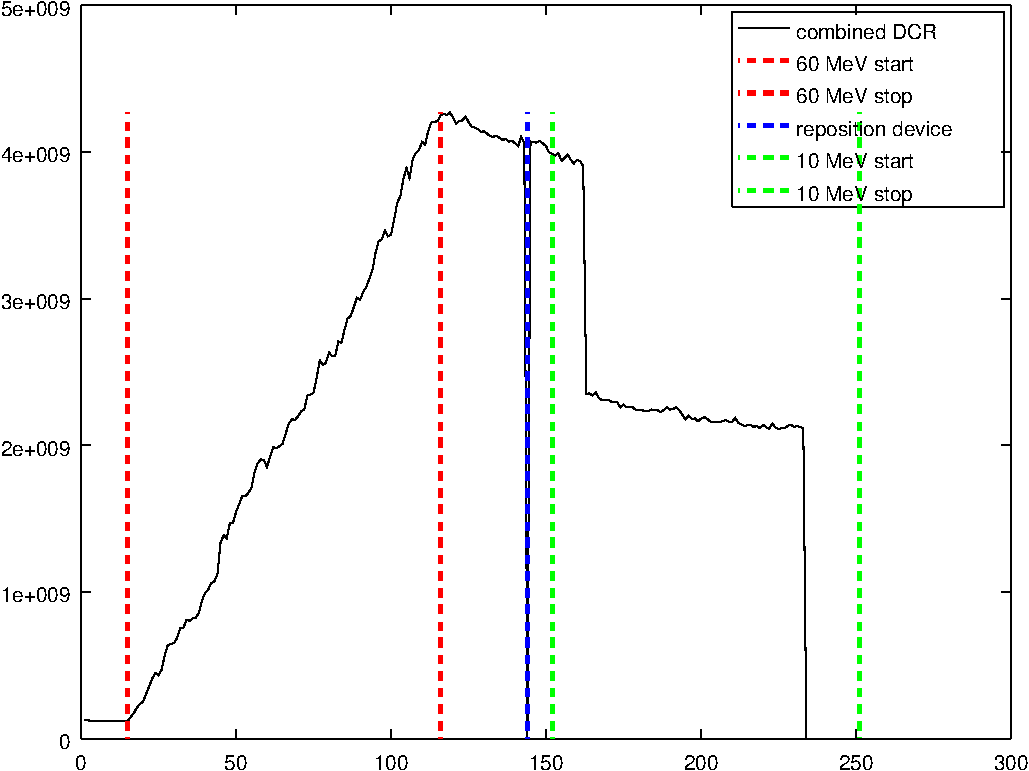
\includegraphics[width=0.6\linewidth]{fig/count_vs_time_sum_all.pdf}
\caption{The amount of DCR for the sum of all SPADs combined as a function of time}
\label{fig:count_vs_time_sum_all}
\end{figure}


\begin{figure}[h]
\centering
	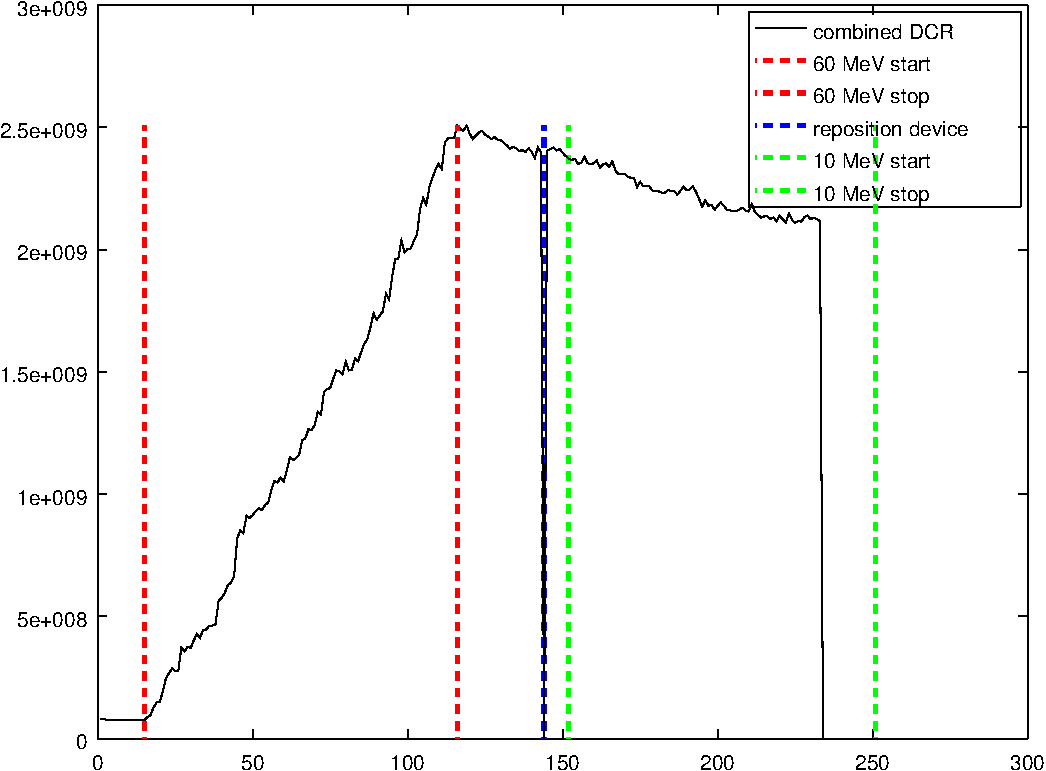
\includegraphics[width=0.6\linewidth]{fig/count_vs_time_sum_some.pdf}
\caption{The amount of DCR for the sum of $75\,\%$ of SPADs combined as a function of time. The left-out $25\,\%$ are the SPADs that broke down at the 165 minute mark}
\label{fig:count_vs_time_sum_some}
\end{figure}

\Cref{fig:bars} shows the accumulative number of counts for individual SPADs. This plot illustrates that the contribution in DCR varies wildly across different SPADs. It also shows that the second half of the SPADs seem te behave at a much lower count than the first half, which is something that needs to be looked at.

\begin{figure}[h]
\centering
	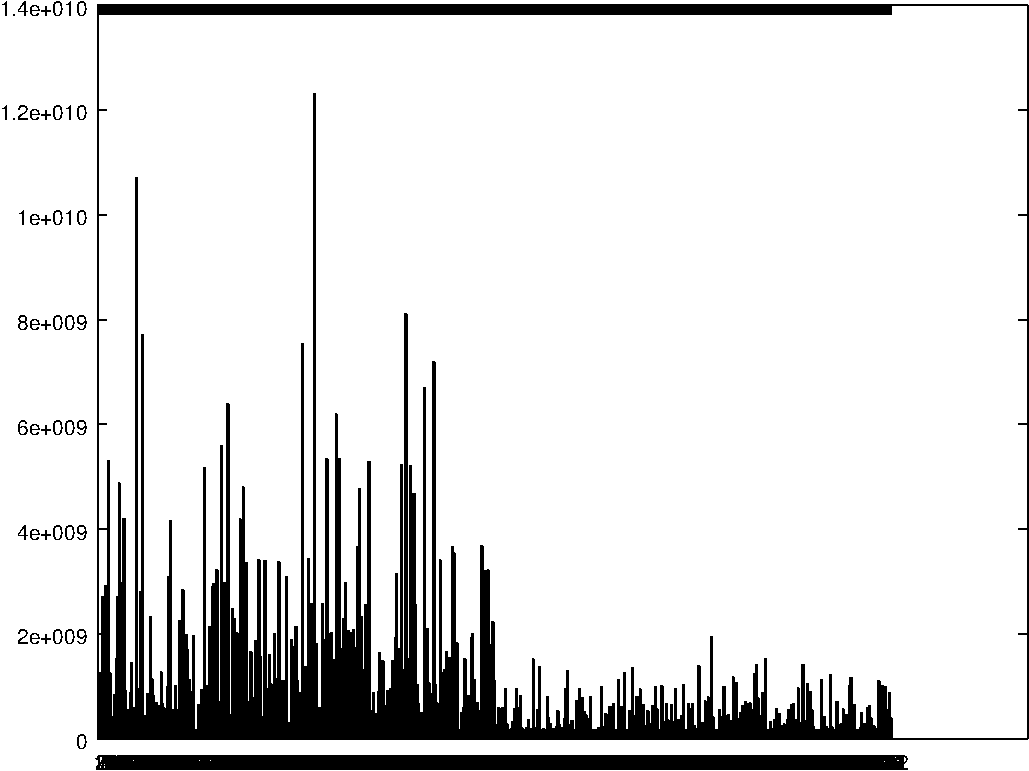
\includegraphics[width=0.6\linewidth]{fig/bars.pdf}
\caption{accumulative number of counts for the entire experiment for individual SPADs}
\label{fig:bars}
\end{figure}

\Cref{fig:spad_high}, \cref{fig:spad_mid} and \cref{fig:spad_low} show the individual DCR as a function of time for three SPADs in the high, mid and low segment respectively. The segments are sorted by how much counts a SPAD accumulated over the course of the entire test. Note that the individual SPADs don't show the same trend as the sum of all SPADs. The individual SPADs get damaged at arbitray points in time, and anneal at a certain point in time. 

\begin{figure}[h]
\centering
	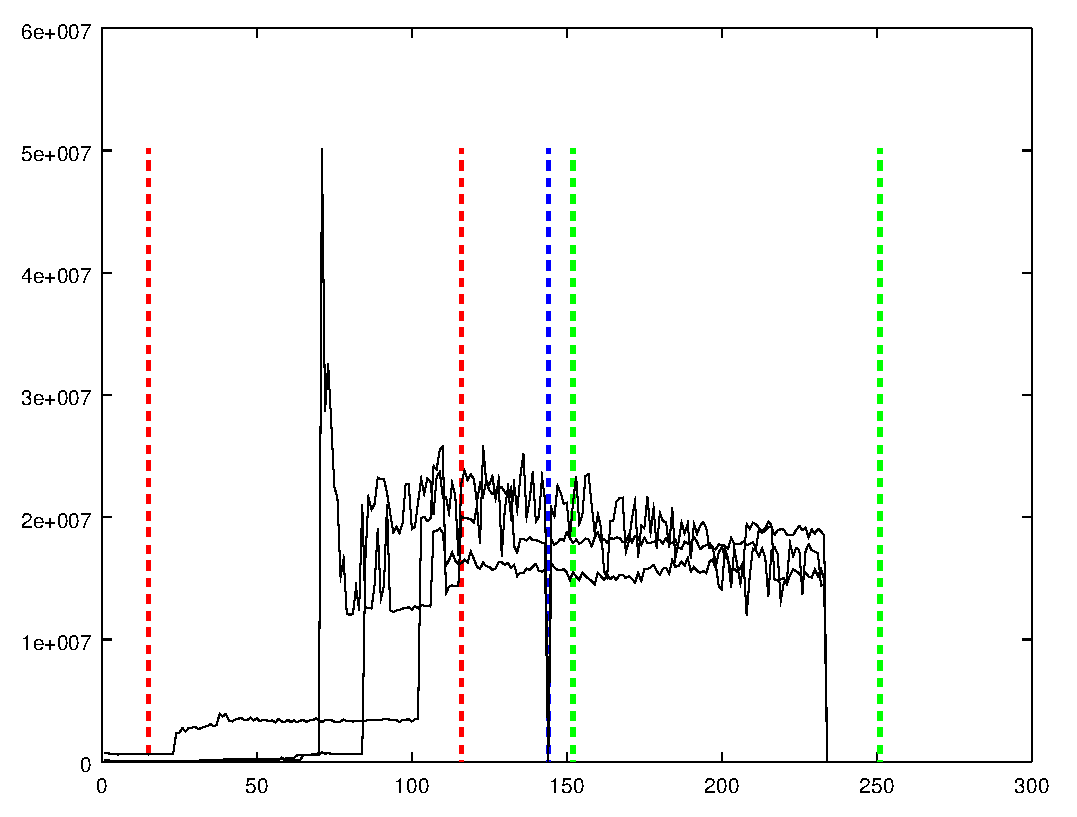
\includegraphics[width=0.6\linewidth]{fig/spad_high.eps}
\caption{three SPADs from that are in picked from the $33\,\%$ SPADs with the highest contribution to noise}
\label{fig:spad_high}
\end{figure}


\begin{figure}[h]
\centering
	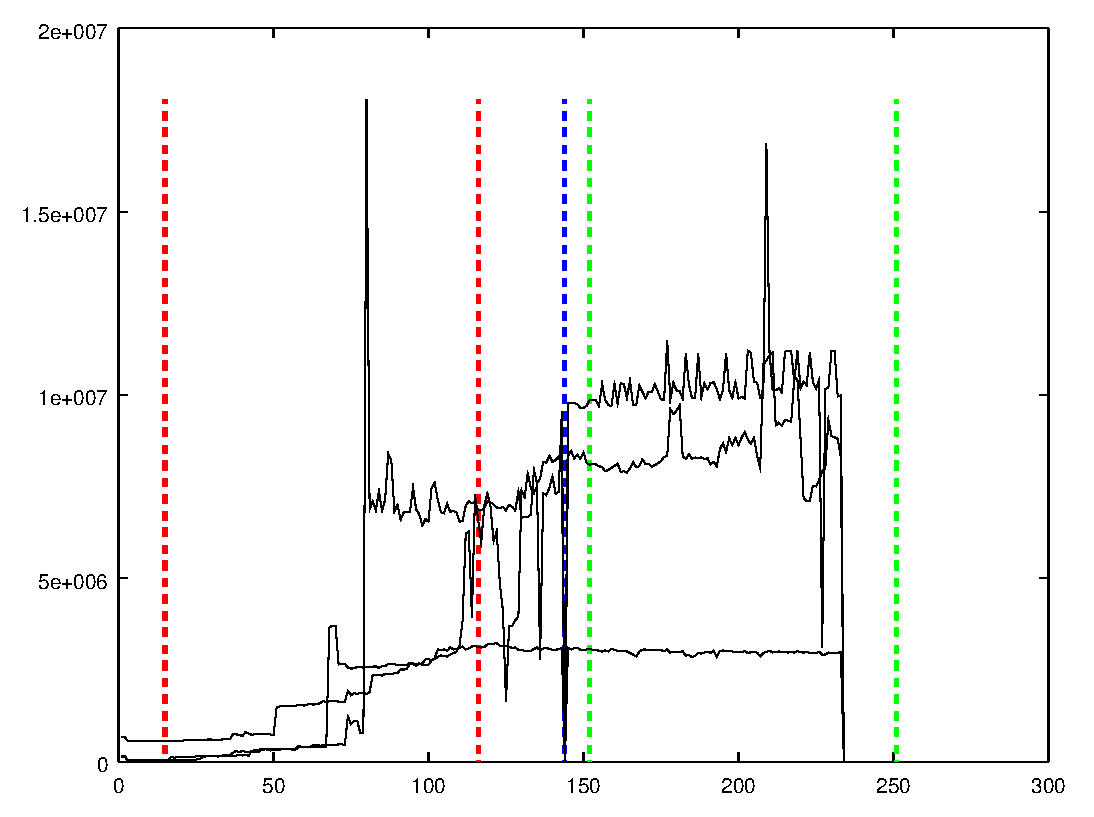
\includegraphics[width=0.6\linewidth]{fig/spad_mid.eps}
\caption{three SPADs from that are in picked from the $33\,\%$ SPADs with the most average contribution to noise}
\label{fig:spad_mid}
\end{figure}


\begin{figure}[h]
\centering
	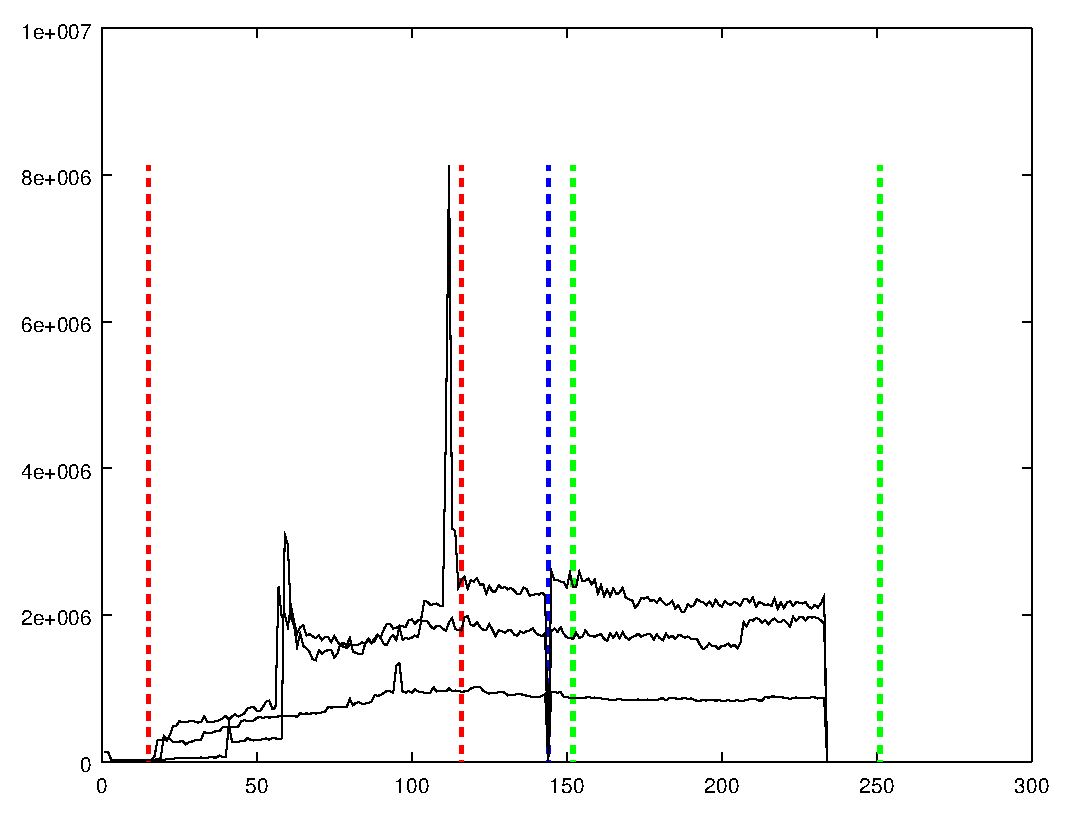
\includegraphics[width=0.6\linewidth]{fig/spad_low.eps}
\caption{three SPADs from that are in picked from the $33\,\%$ SPADs with the lowest  contribution to noise}
\label{fig:spad_low}
\end{figure}

\Cref{fig:sigmoid_sweep} shows the spread of DCR for single SPADs at different points in time. The behavior is consistent with the results shown in \cref{fig:count_vs_time_sum_all}. Note that after approximately 165 minutes $25\,\%$ of the SPADs stop working, which is the reason why the black line starts at $25\,\%$.

\begin{figure}[h]
\centering
	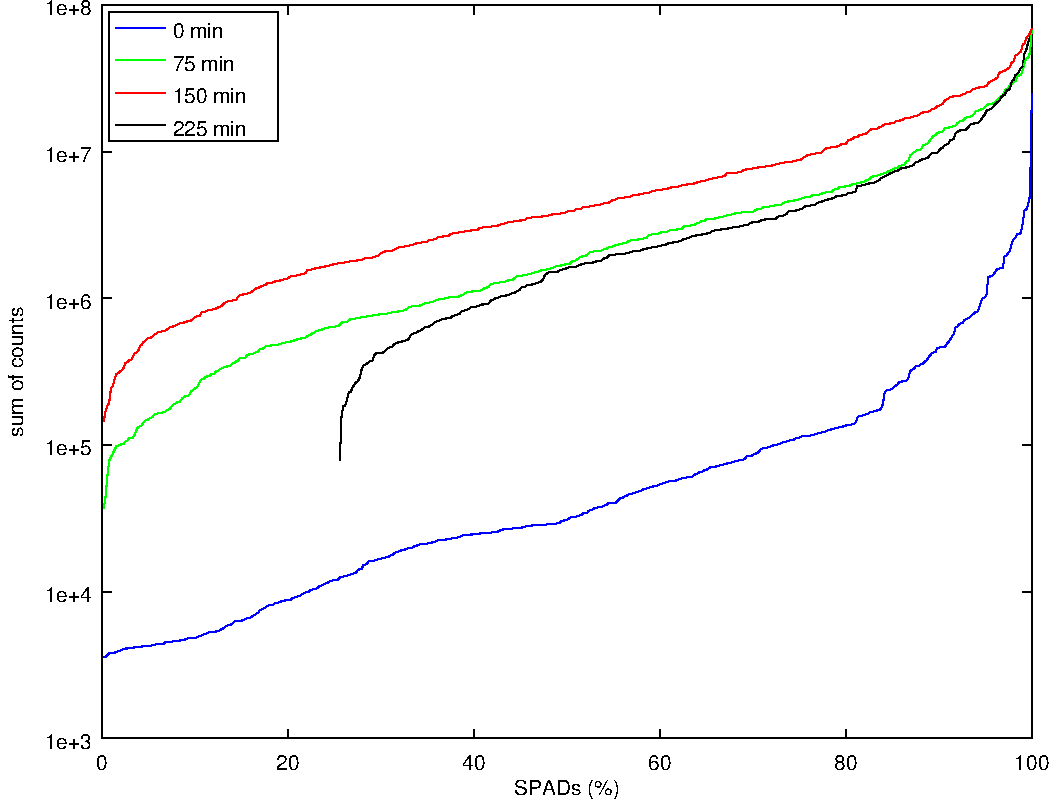
\includegraphics[width=0.6\linewidth]{fig/sigmoid_sweep.pdf}
\caption{distribution of DCR over individual SPADs at different time frames. After the 165 minute mark $25\,\%$ of SPADs stop working, which is why the black line starts later at $25\,\%$}
\label{fig:sigmoid_sweep}
\end{figure}


The results of the test are in line with until the 150 minute mark, but afterwards the reaction to the $10\,MeV$ beam is odd. The break down at 165 minutes and 250 minutes indicate damage in the readout circuit. This is a feasible explanation for the events as it is known that the $10\,MeV$ can be very damaging to these types of cicruitry. This would mean that the protection provided for the ROIC and FPGA where insufficient. There are two possible explanations for the observation that the SPADs are not affected by the $10\,MeV$ beam that will be listed here. The first explanation, is that the SPADs at this particular $0.18\,\mu m$ technology are not affected by the $10\,MeV$ as opposed to their $0.35\,\mu m$ counterpart. The second explanation is that something went wrong during the setup of the $10\,MeV$ beam test, which caused the beam to aim for the ROIC and FPGA instead of the SPAD array. 

Considering only the effect of the $60\,MeV$ beam, and especially the behavior observed in \cref{fig:count_vs_time_sum_some}, show a very interesting trend where the change in DCR seems to be a linear relationship with the amount of radiation it is exposed to. Both the periods between 10 and 120 minutes, and between 120 and 240 minutes show a very constant slope. This means that not only the amount, but also the time over which the radiation dose is accumulated graetly affects the DCR of the device. This property should be further investigated and compared to the circumstances at Europa.
